\chapter{Experiments Setup}
\label{chapter6}

\section{Super-Mega-Bot Mobile Base}
\begin{figure}[h]
	\begin{center} 
		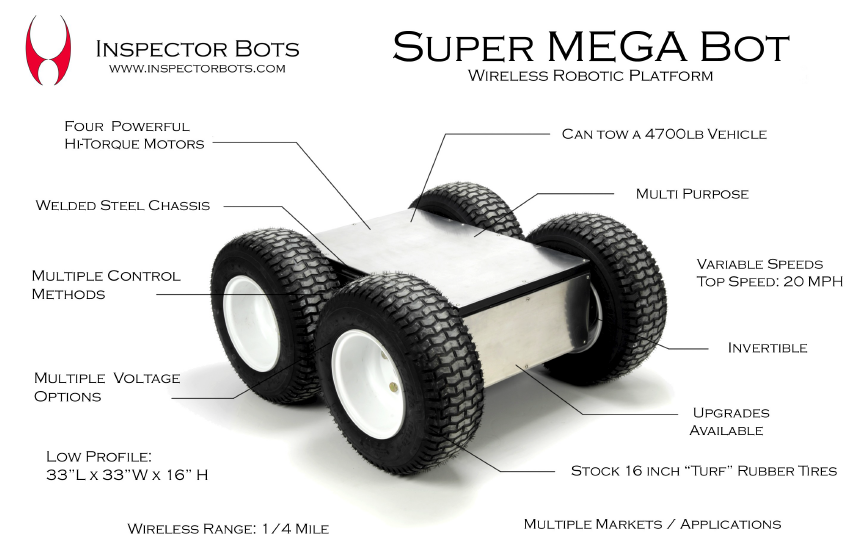
\includegraphics[scale=0.6]{SuperMegaBot}
		\centering
		\label{fig:SuperMegaBot} 
	\end{center}
\end{figure}
PAYLOAD

NON CI STA LA CONTROL BOX DELL'UR5


The InspectorBots Super Mega Bot robot platform is a Heavy-Duty, All-Terrain, 4WD Robotic Platform. It is a very rugged, Indoor/outdoor, remotely operated platform and can be fitted with a variety of sensors, cameras and equipment. The MEGA Bot has been designed to be Modular and Reconfigurable, so an end user can swap out various modules. There are several methods available to control the SMB including: RC radio, Analog Joystick, Wireless Modem, or Microcomputer.\\
Its base model comes with:\\
•	Chassis: Powder Coated Steel and Aluminum \\
•	Dimensions: 84cm L x 84cm W x 40.64cm H, Weight: 109 kg\\
•	Drive: Four Electric Motors\\
•	Load Capacity: 113,5 kg\\
•	Speed Controllers: RoboteQ 2x VDC2450\\
•	Speed: 0-16 km/h \\
•	Suspension: Rigid\\
•	Tires: Interchangeable, Pneumatic, 40.64cm Diameter Turf Tires\\
\url{https://www.youtube.com/watch?v=3X8IWnR1QDI}
\begin{figure}[h]
	\begin{center} 
		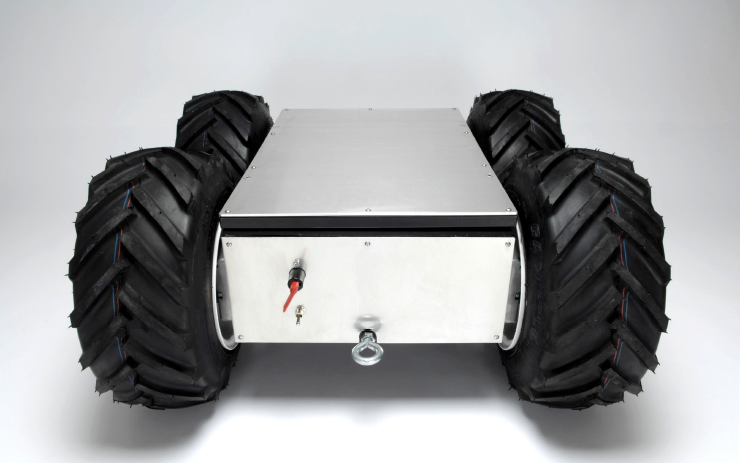
\includegraphics[scale=0.6]{SuperMegaBot1}
		\centering
		\label{fig:SuperMegaBot1}
	\end{center}
\end{figure}

\section{UR5 Manipulator}
The UR5 is a robot developed by Universal Robots, a Danish company. According to the company the key benefits of their robots are that they are light weight, safe and easy to use. The robotic arm is regarded as safe, because it will stop acting as soon as the robot hits an object sensed by a force sensor in one of the joints. UR5 is ideal for automating low-weight processing tasks like picking, placing and testing. The medium-sized robot arm is easy to program, fast to set up and, always according to UR, offers one of the fastest payback times in the industry.

\begin{figure}[htbp]
	\begin{center} 
		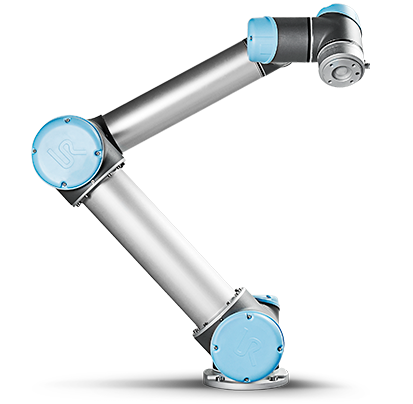
\includegraphics[scale=0.4]{UR5}
		\centering
		\label{fig:UR5} 
	\end{center}
\end{figure}

In the following table the specifications given by Universal Robots are stated. 
\begin{table}
	\begin{tabular}{p{4cm} | p{3cm} p{3cm}}
		\hline
		Performance & \multicolumn{2}{l}{ } \\
		\hline \hline
		Repeatibility & \multicolumn{2}{l}{$\pm$ 0.1 mm} \\
		Ambient temperature range & \multicolumn{2}{l}{0-50°} \\
		Power Consumption  & \multicolumn{2}{l}{Min 90W, Typical 150W, Max 325W} \\
		Collaboration operation & \multicolumn{2}{l}{15 advanced adjustable safety functions} \\
		\hline \hline
		Specifications & \multicolumn{2}{l}{ }\\
		\hline \hline 
		Payload & \multicolumn{2}{l}{5 kg} \\
		Reach & \multicolumn{2}{l}{850 mm} \\
		Degrees of freedom & \multicolumn{2}{l}{6 rotating joints} \\
		Programming & \multicolumn{2}{l}{Polyscope graphical user interface on 12 inch touchscreen} \\
		\hline \hline
		Movement & & \\
		\hline 
		& Working range & Maximum speed \\
		\hline \hline
		Base & $\pm$ 360°  & $\pm$ 180°/sec \\
		Shoulder & $\pm$ 360° & $\pm$ 180°/sec \\
		Wrist1 & $\pm$ 360° & $\pm$ 180°/sec \\
		Wrist2 & $\pm$ 360° & $\pm$ 180°/sec \\
		Wrist3 & $\pm$ 360° & $\pm$ 180°/sec \\
		Typical tool & & 1m/sec \\
		\hline \hline
		Physical & \multicolumn{2}{l}{ }\\
		\hline \hline
		Footprint & \multicolumn{2}{l}{$\o$ 149mm} \\
		Materials & \multicolumn{2}{l}{Aluminium, PP Plastics} \\
		Weight (with cable) & 18.4 kg 
	\end{tabular}
\end{table}

\section{ADDAMS}
SCRITTA MALISSIMO: The goal of this mobile manipulator is to fill the gap between small and large production. Indeed small production companies could not have the need to have a static robot, still needing an automatized process.  Maybe they also don’t have the money for the sensors needed to accomplish things. So there is the need of a robot able to substitute a person in the process but still having a user interface. 
\subsection{Mission}
\subsection{Sensors}
\section{MPC}
\subsection{Kinematic model based}
\subsection{Dynamic model based}
